\PassOptionsToPackage{unicode}{hyperref}
\documentclass[aspectratio=1610, 9pt]{beamer}

\usetheme{vertex}

\usepackage[ngerman]{babel}

\usepackage{siunitx}

\usepackage{grffile}
\usepackage{graphicx}
\usepackage{tikz}
\usetikzlibrary{calc}

\usepackage{hyperref}
\usepackage{bookmark}


\title{Farbwahrnehmung und Datenvisualisierung}
\author[maxnoe]{Maximilian Nöthe}
\date[SoAk19]{PeP et al. Sommerakademie 2019}
\institute{PeP et Al.}

\begin{document}
\maketitle

\begin{frame}[t]{Überblick}
  \tableofcontents
\end{frame}

\section{Menschliche Farbwahrnehmung}
\bumper{Menschliche Farbwahrnehmung}

\begin{frame}[c]{Geschichte}
  \begin{columns}[onlytextwidth]
    \hfill
    \begin{column}{0.59\textwidth}
      \begin{itemize}
        \item Erste physiologische Versuche durch Johann Wolfgang von Goethe (Zur Farbenlehre, 1810) \\
        \item Dreifarbentheorie (Young \& v. Helmholtz, 1804 / 1850)
        \item Gegenfarbtheorie (Ewald Hering 1878) \\
          \begin{tabular}{r @{${}⟷  {}$} l}
            blau & gelb \\
            rot & grün \\
            hell & dunkel \\
          \end{tabular}
        \item Erster Nachweis der Zapfen (Svaetichin, 1956) 
      \end{itemize}
    \end{column}
    \hfill%
    \begin{column}{0.39\textwidth}
      \hfill%
      \vfill%
      \centering
      \only<1>{%
        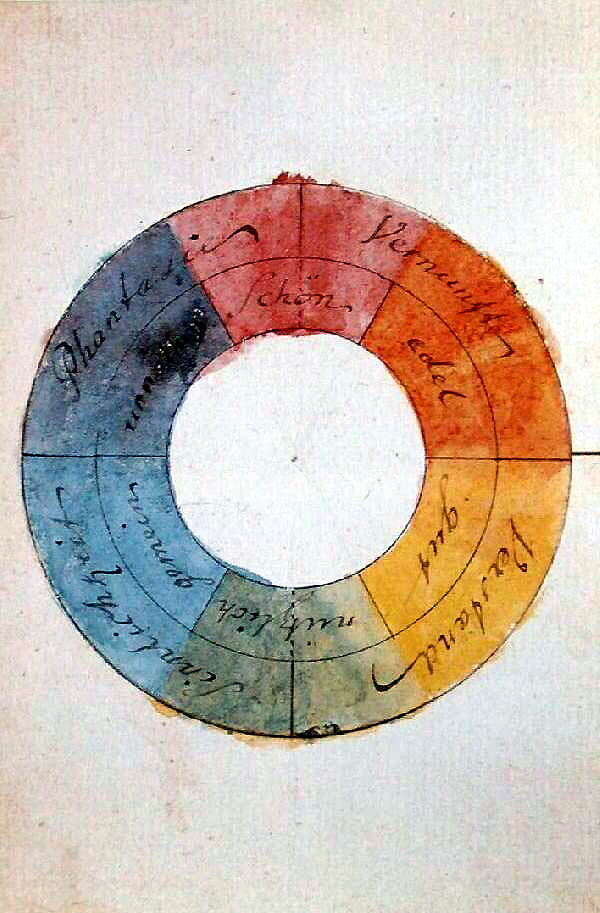
\includegraphics[width=\linewidth, height=0.90\textheight, keepaspectratio]{images/goethe_farbenkreis.jpg}

        [Goethe, 1809]
      }%
      \only<2>{%
        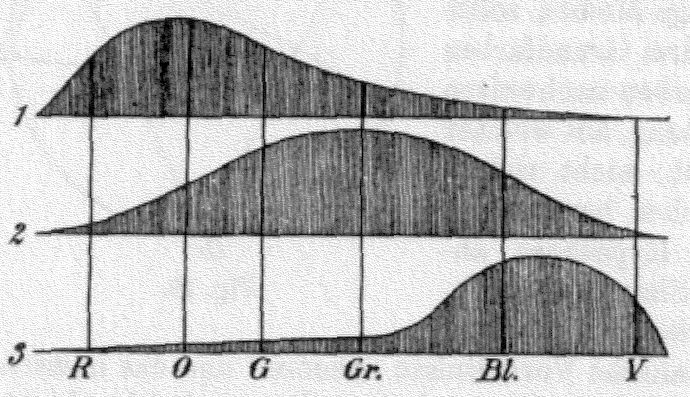
\includegraphics[width=\linewidth]{images/YoungHelm.jpg}

        [v. Helmholtz, 1894]
      }%
      \vfill%
    \end{column}%
  \end{columns}%
\end{frame}

\begin{frame}[c, plain]
  \centering
  \begin{tikzpicture}[shift=(current page.center), remember picture, overlay]
    \fill[color=green] (0, 0) rectangle (-0.2\textwidth, 0.2\textwidth);
    \fill[color=yellow] (0, 0) rectangle (0.2\textwidth, 0.2\textwidth);
    \fill[color=blue] (0, 0) rectangle (-0.2\textwidth, -0.2\textwidth);
    \fill[color=red] (0, 0) rectangle (0.2\textwidth, -0.2\textwidth);
    \fill[color=black] (0, 0) circle (0.02\textwidth);
  \end{tikzpicture}
\end{frame}

\begin{frame}[c, plain]
  \begin{tikzpicture}[remember picture, overlay, shift=(current page.center)]
    \fill[color=black] (0, 0) circle (0.02\textwidth);
  \end{tikzpicture}
\end{frame}


\begin{frame}[t]{Zapfen}
  \includegraphics{build/plots/cone_response.pdf} 
\end{frame}


\section{15 Minuten Einführung in Farbtheorie}

\section{Datenvisualisierung}
\bumper{Datenvisualisierung}

\begin{frame}{Warum?}

  {
    \tiny
    \input{build/img.tex}
  }

  \only<2->{%
    \begin{tikzpicture}[remember picture, overlay, shift=(current page.center)]
      \node[anchor=south east] (A) at (0.5\textwidth, -0.5\textheight) {{
        \includegraphics[height=4cm]{build/plots/u_sw.png}
      }};
    \end{tikzpicture}
  }
\end{frame}

\end{document}
